\Subhead{2.4.1}{Механические и электрические цепочки. Акустические и оптические фононы. Полосы пропускания и непрозрачности}

Для одинаковых масс $m$, шага $a$ и пружин жёсткости $K$ имеем
\begin{equation}
 m\ddot u_n=K(u_{n+1}-2u_n+u_{n-1}).
\end{equation}
Подстановка $u_n=U\exp[\ii(kna-\omega t)]$ даёт $\omega^2=(4K/m)\sin^2(ka/2)$. Независимые волновые числа можно выбрать в первой зоне Бриллюэна $|k|\leq\pi/a$. При $ka\ll1$ получаем звук со скоростью $a\sqrt{K/m}$; у края зоны групповая скорость обращается в нуль.

Два различных атома в ячейке дают две ветви. Для масс $m_1,m_2$ и периода ячейки $a$
\begin{equation}
 \omega_\pm^2=K\left(\frac1{m_1}+\frac1{m_2}\right)
 \pm K\sqrt{\left(\frac1{m_1}+\frac1{m_2}\right)^2-
 \frac4{m_1m_2}\sin^2\frac{ka}{2}}.
\end{equation}
Нижняя ветвь акустическая: при $k\to0$ подрешётки движутся совместно и $\omega\to0$. Верхняя — оптическая: относительное движение имеет ненулевую частоту при $k=0$. Название связано с возможным взаимодействием с электромагнитным полем в полярных кристаллах, а не с обязательной оптической частотой любой цепочки.

В электрической LC-цепочке аналогичная дисперсия получается из дискретных законов Кирхгофа: $m$ заменяется индуктивностью, упругая связь — обратной ёмкостью при соответствующем выборе координаты. Континуальный предел допустим только для длин волн, много больших шага; он теряет край зоны и запрещённые полосы.
\begin{center}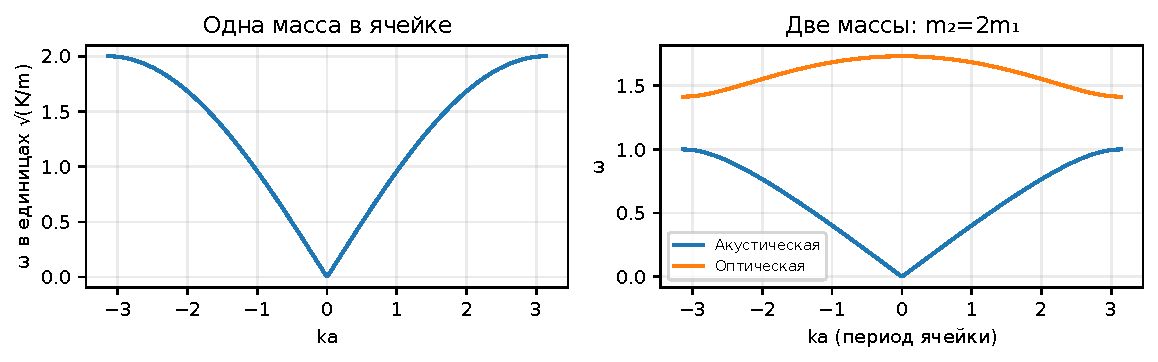
\includegraphics[width=0.8\linewidth]{figures/bands.pdf}\end{center}

